\begin{figure}
  \centering

  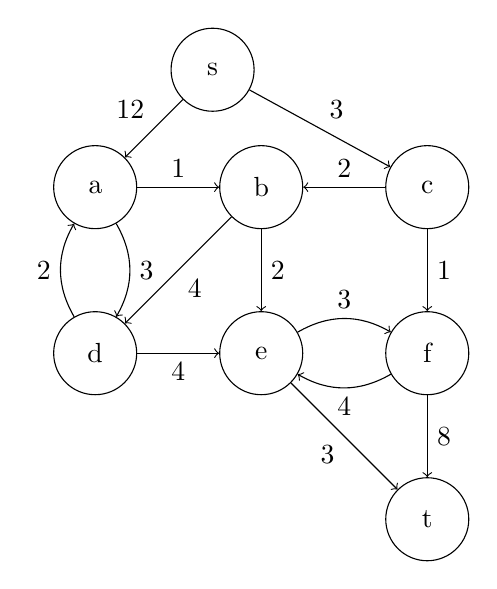
\begin{tikzpicture}[->, auto, node distance=6em, main node/.style={circle, draw, minimum size=3em}]
    \node (s) [main node] {s};
    \node (a) [main node, below left of=s] {a};
    \node (b) [main node, right of=a] {b};
    \node (c) [main node, right of=b] {c};
    \node (d) [main node, below of=a] {d};
    \node (e) [main node, right of=d] {e};
    \node (f) [main node, right of=e] {f};
    \node (t) [main node, below of=f] {t};

    \path[every node]
    (s) edge node [above left] {12} (a)
    (s) edge node {3} (c)
    (a) edge node {1} (b)
    (c) edge node [above] {2} (b)
    (a) edge [bend left] node {3} (d)
    (d) edge [bend left] node {2} (a)
    (b) edge node {4} (d)
    (d) edge node [below] {4} (e)
    (b) edge node {2} (e)
    (c) edge node {1} (f)
    (e) edge [bend left] node {3} (f)
    (f) edge [bend left] node {4} (e)
    (e) edge node [below left] {3} (t)
    (f) edge node {8} (t)
    ;
  \end{tikzpicture}

  \caption{Graph $G$}\label{fig:dijkstra}
\end{figure}